% Update slides, version 3 (19 Nov 2026): memory / speed-up tests of the
% kinetic-only solver, job 2877888 on Pitagora: output diagnostics nu_s/nu_D
% off AND the passing-orbit metric table of the grids no longer stored
% (computed on the fly when there are no trapped orbits).
% Versions kept for comparison:
%   v1  job 2859315   figures in v1_2859315/
%   v2  job 2877157   update_frames.tex, figures in v2_2877157/
%   v3  job 2877888   this file, figures in v3_2877888/
% Figures: make_update_plots.py <DATA> --out v3_2877888.
% Include with % Update slides, version 3 (19 Nov 2026): memory / speed-up tests of the
% kinetic-only solver, job 2877888 on Pitagora: output diagnostics nu_s/nu_D
% off AND the passing-orbit metric table of the grids no longer stored
% (computed on the fly when there are no trapped orbits).
% Versions kept for comparison:
%   v1  job 2859315   figures in v1_2859315/
%   v2  job 2877157   update_frames.tex, figures in v2_2877157/
%   v3  job 2877888   this file, figures in v3_2877888/
% Figures: make_update_plots.py <DATA> --out v3_2877888.
% Include with % Update slides, version 3 (19 Nov 2026): memory / speed-up tests of the
% kinetic-only solver, job 2877888 on Pitagora: output diagnostics nu_s/nu_D
% off AND the passing-orbit metric table of the grids no longer stored
% (computed on the fly when there are no trapped orbits).
% Versions kept for comparison:
%   v1  job 2859315   figures in v1_2859315/
%   v2  job 2877157   update_frames.tex, figures in v2_2877157/
%   v3  job 2877888   this file, figures in v3_2877888/
% Figures: make_update_plots.py <DATA> --out v3_2877888.
% Include with % Update slides, version 3 (19 Nov 2026): memory / speed-up tests of the
% kinetic-only solver, job 2877888 on Pitagora: output diagnostics nu_s/nu_D
% off AND the passing-orbit metric table of the grids no longer stored
% (computed on the fly when there are no trapped orbits).
% Versions kept for comparison:
%   v1  job 2859315   figures in v1_2859315/
%   v2  job 2877157   update_frames.tex, figures in v2_2877157/
%   v3  job 2877888   this file, figures in v3_2877888/
% Figures: make_update_plots.py <DATA> --out v3_2877888.
% Include with \input{update_frames_v3} (update_2026-11-19.tex).

% ---------------------------------------------------------------------
\begin{frame}{Recent changes}
    \begin{itemize}
        \item \textbf{Memory distributed across MPI ranks}
        \begin{itemize}
            \item collision quantities ($\ln\Lambda$, $\nu_s$, $\nu_D$, $\nu_\parallel$) split by radius,
                  following the PETSc rows of $f_\mathrm{hot}$, $f_\mathrm{re}$
            \item partial derivatives no longer stored: computed cell by cell when needed
            \item kinetic operators (transient weights, advection/diffusion coefficients,
                  interpolation coefficients) stored only on the $\xi$-lines a rank owns
        \end{itemize}
        \item \textbf{Solver now handles the current-quench (CQ) snapshots}
        \begin{itemize}
            \item MIRadialBJ: each radius block uses BoomerAMG with a
                  Euclid ILU(1) smoother by default
            \item CQ at 29\,ms ($E \approx 31$\,V/m): failed with ILU(0),
                  now converges in 11 outer iterations
        \end{itemize}
        \item \textbf{Kinetic-only fluid unknowns} ($n_\mathrm{re}$, $j$, $n_\mathrm{tot}$)
              initialised by DREAM's own equations, then kept fixed
        \item \textbf{Memory and timing per stage} logged by \texttt{dreami}
              (\texttt{-dream\_log\_memory}) + batch script and summary
        \item \textbf{Replicated memory reduced}
        \begin{itemize}
            \item output diagnostics $\nu_s$, $\nu_D$ (full momentum grids) no longer saved: $-286$\,MB
            \item grid metric $\sqrt{g}$ computed when needed, not stored per cell
                  (cylindrical: no trapped orbits): $-260$\,MB
        \end{itemize}
    \end{itemize}
\end{frame}

% ---------------------------------------------------------------------
\begin{frame}{Correctness check}
    Reference: first kinetic-only version (serial) and unmodified DREAM, same settings
    \vspace{0.5em}
    \begin{center}
    \begin{tabular}{lcc}
        \hline
        comparison & $f_\mathrm{hot}$ & $f_\mathrm{re}$ \\
        \hline
        current code vs first kinetic-only version & $4\times10^{-9}$ & $1\times10^{-7}$ \\
        full DREAM (particle source off) vs first version & $6\times10^{-10}$ & $2\times10^{-14}$ \\
        \hline
    \end{tabular}
    \end{center}
    \vspace{0.5em}
    \begin{itemize}
        \item differences at the level of the iterative solver tolerance
        \item collision quantities: 1 rank vs $N$ ranks identical (difference exactly 0)
        \item only physics difference with full DREAM: the $f_\mathrm{hot}$ particle source,
              not included in kinetic-only mode ($\sim 8\times10^{-4}$ per step in $f_\mathrm{hot}$)
    \end{itemize}
\end{frame}

% ---------------------------------------------------------------------
\begin{frame}{Memory and speed-up test: setup}
    \begin{itemize}
        \item 3 snapshots of the ITER disruption: injection start, injection end, CQ final
        \item resolution level L2:
        \begin{itemize}
            \item hot-tail grid $500 \times 64$, runaway grid $300 \times 400$ ($p \times \xi$)
            \item $N_r = 11$ radii $\Rightarrow \approx 1.7$\,M unknowns
        \end{itemize}
        \item 1 time step, cylindrical geometry, linear solver MIRadialBJ
        \item Pitagora (CINECA), 1 node (256 cores), $n = 1, 11, 22, 44, 88, 176$ MPI ranks,
              2 runs each (fastest kept)
        \item measured per rank:
        \begin{itemize}
            \item resident memory at each stage (construction, matrix, solve)
            \item size of each distributed data structure
            \item time of the time loop, of the solve and of the whole run
        \end{itemize}
    \end{itemize}
\end{frame}

% ---------------------------------------------------------------------
\begin{frame}{Memory per rank}
    \begin{columns}[T]
        \begin{column}{0.58\textwidth}
            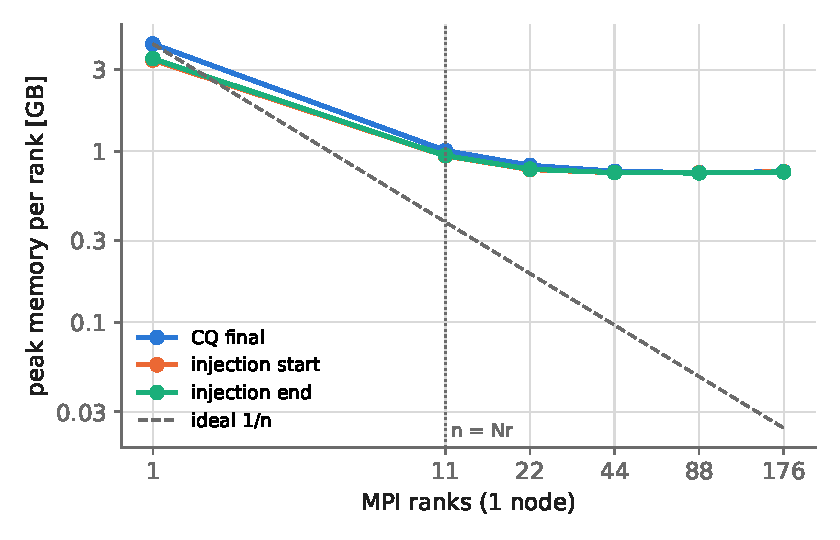
\includegraphics[width=\linewidth]{v3_2877888/fig_memory_scaling}
        \end{column}
        \begin{column}{0.42\textwidth}
            \small
            \begin{itemize}
                \item CQ final: 4.34\,GB (1 rank) $\to$ 1.03\,GB (11) $\to$ 0.78\,GB (176)
                \item \textbf{plateau at $\approx 0.78$\,GB} from 44 ranks on
                \item same behaviour for the 3 snapshots
                \item the distributed parts do scale:
                \begin{itemize}
                    \item solve (incl.\ AMG setup) 2.83\,GB $\to$ 33\,MB
                    \item PETSc matrix 463 $\to$ 5\,MB
                    \item coefficients 302 $\to$ 10\,MB
                \end{itemize}
                \item at 176 ranks: $\approx 134$\,GB per node, vs 4.3\,GB serial
            \end{itemize}
        \end{column}
    \end{columns}
\end{frame}

% ---------------------------------------------------------------------
\begin{frame}{Memory: whole run vs construction only}
    \begin{columns}[T]
        \begin{column}{0.58\textwidth}
            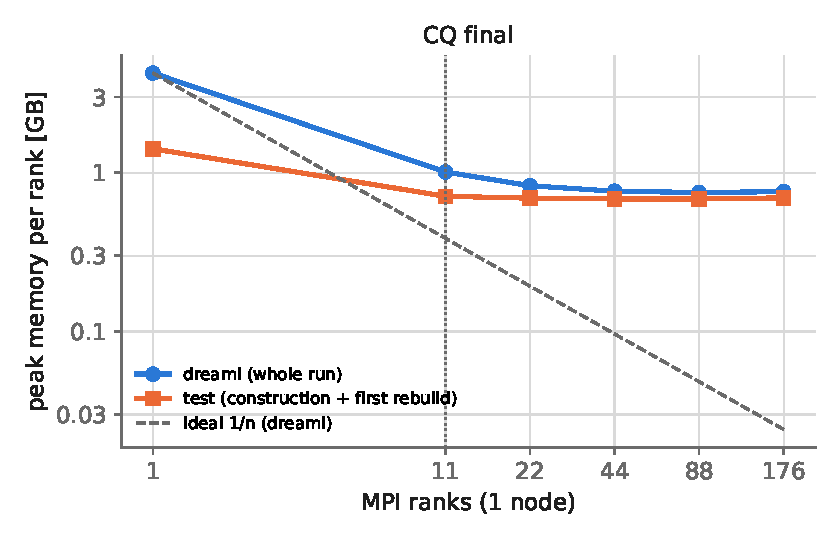
\includegraphics[width=\linewidth]{v3_2877888/memory_CQ_tf}
        \end{column}
        \begin{column}{0.42\textwidth}
            \small
            \begin{itemize}
                \item \textbf{test}: construction + first rebuild, no solve
                \begin{itemize}
                    \item 1.45\,GB $\to$ 0.71\,GB, flat from 11 ranks on
                \end{itemize}
                \item \textbf{dreami}: whole run
                \begin{itemize}
                    \item 4.34\,GB $\to$ 0.78\,GB
                \end{itemize}
                \item the gap between the two (the solve) shrinks with $n$:
                      the solver memory is distributed
                \item the plateau is already there after the construction:
                      the replicated data is created when the simulation is built
            \end{itemize}
        \end{column}
    \end{columns}
\end{frame}

% ---------------------------------------------------------------------
\begin{frame}{Where the memory of a rank goes}
    \begin{columns}[T]
        \begin{column}{0.56\textwidth}
            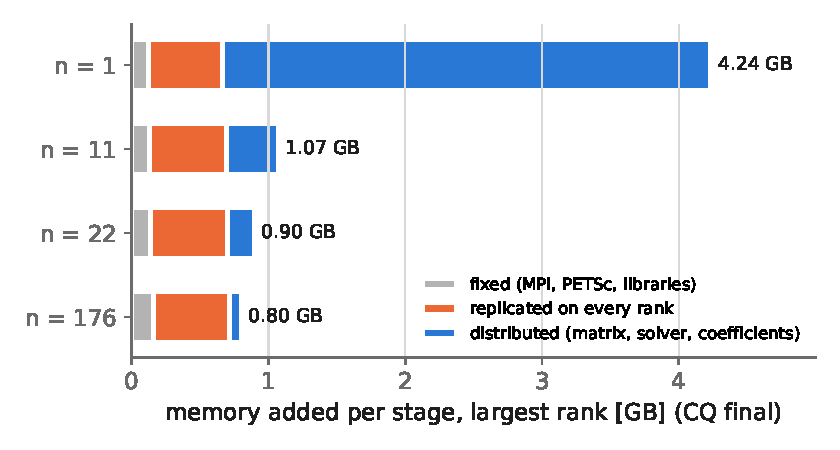
\includegraphics[width=\linewidth]{v3_2877888/fig_memory_breakdown}
        \end{column}
        \begin{column}{0.44\textwidth}
            \small
            Still \textbf{replicated} on every rank ($\approx 0.49$\,GB):
            \vspace{0.3em}

            \begin{tabular}{lrr}
                \hline
                & now & before \\
                \hline
                runaway grid data & 168\,MB & 374\,MB \\
                system setup (vectors) & 142\,MB & 142\,MB \\
                unknowns ($f$ history) & 71\,MB & 72\,MB \\
                equation terms & 64\,MB & 64\,MB \\
                hot-tail grid data & 46\,MB & 100\,MB \\
                output quantities & 0\,MB & 286\,MB \\
                \hline
            \end{tabular}
            \vspace{0.5em}

            Grid data: the metric $\sqrt{g}$ (one array per cell) is now
            computed when a bounce average needs it.
            Output: $\nu_s$, $\nu_D$ diagnostics removed
            (the solver's own $\nu_s$, $\nu_D$ are distributed)
            \vspace{0.3em}

            Above 22 ranks this is almost all of a rank's memory
        \end{column}
    \end{columns}
\end{frame}

% ---------------------------------------------------------------------
\begin{frame}{Speed-up}
    \begin{columns}[T]
        \begin{column}{0.5\textwidth}
            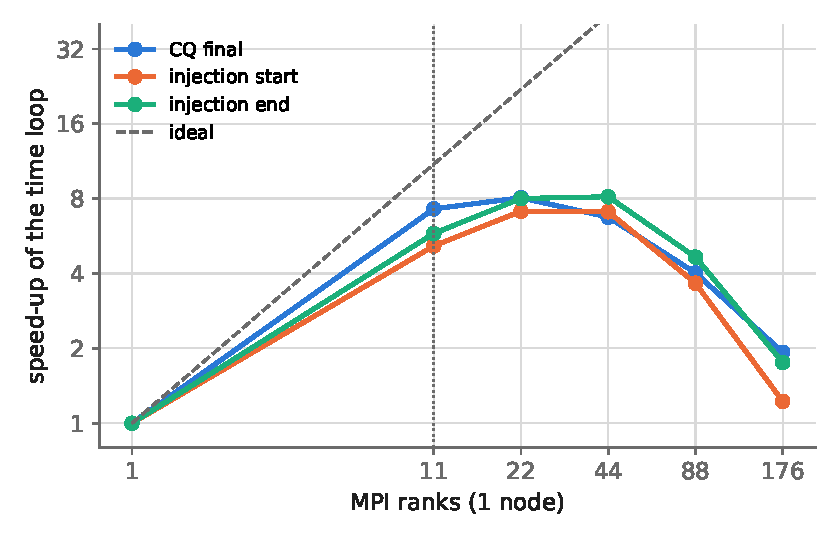
\includegraphics[width=\linewidth]{v3_2877888/fig_speedup}
            \centering{\footnotesize time loop, 3 snapshots}
        \end{column}
        \begin{column}{0.5\textwidth}
            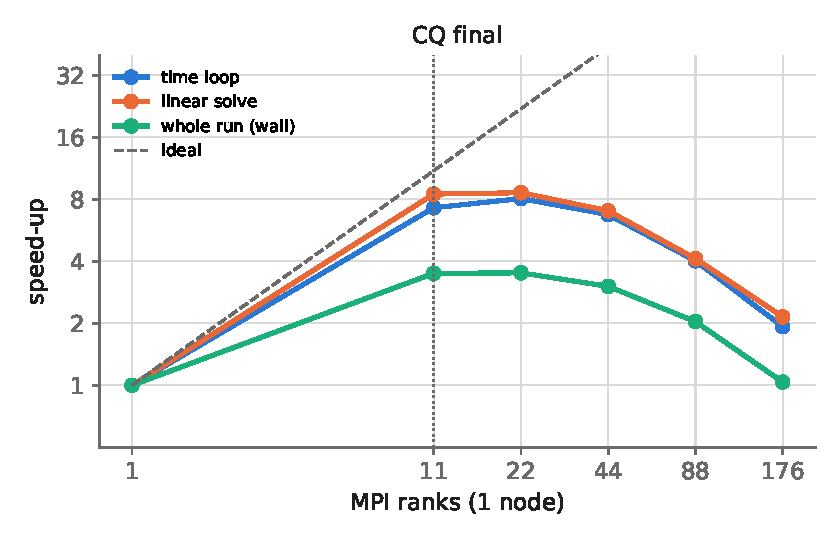
\includegraphics[width=\linewidth]{v3_2877888/speedup_CQ_tf}
            \centering{\footnotesize CQ final: loop, linear solve, whole run}
        \end{column}
    \end{columns}
    \vspace{0.3em}
    \small
    \begin{itemize}
        \item time loop: best at 22--44 ranks, $\approx 7$--$8\times$ (CQ final: 11.6\,s $\to$ 1.44\,s at 22 ranks)
        \item for $n > N_r$ each radius block is split over $n/N_r$ ranks:
              AMG/ILU setup dominated by communication
        \item whole run: at most $3.5\times$ (11--22 ranks), $1.0\times$ at 176 ranks
    \end{itemize}
\end{frame}

% ---------------------------------------------------------------------
\begin{frame}{Where the time goes (CQ final)}
    \begin{center}
        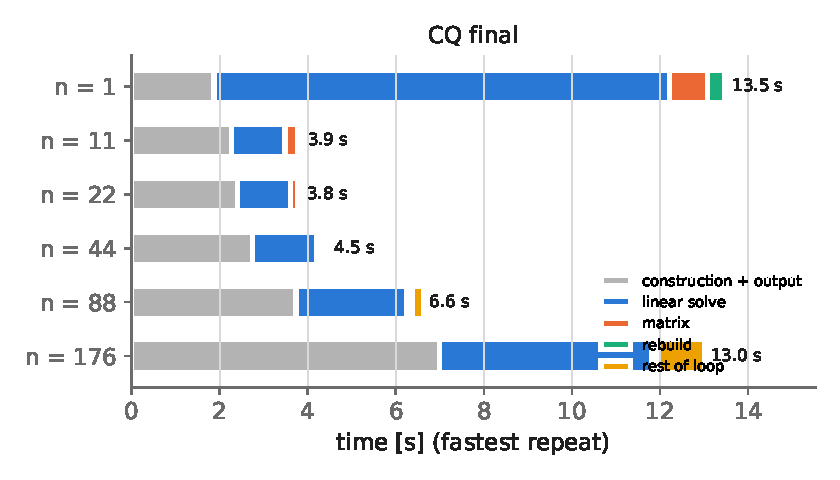
\includegraphics[width=0.85\linewidth]{v3_2877888/time_breakdown_CQ_tf}
    \end{center}
    \small
    \begin{itemize}
        \item 1 rank: 13.5\,s, of which 10.3\,s linear solve and 1.9\,s construction
        \item 22 ranks: 3.8\,s, the solve is down to 1.2\,s, the construction is 2.4\,s
        \item 176 ranks: 13.0\,s, construction 7.0\,s (replicated work, all ranks at the same time)
              and solve 4.8\,s (communication)
        \item \textbf{the construction does not scale}: same cause as the replicated memory
    \end{itemize}
\end{frame}

% ---------------------------------------------------------------------
\begin{frame}{Memory reduction step by step (CQ final, L2, $N_r = 11$)}
    \begin{center}
    \begin{tabular}{lccc}
        \hline
        & v1 & v2 & v3 \\
        & & no $\nu_s$, $\nu_D$ output & + metric on the fly \\
        \hline
        peak per rank, 1 rank      & 4.83\,GB & 4.59\,GB & 4.34\,GB \\
        peak per rank, 11 ranks    & 1.60\,GB & 1.30\,GB & 1.03\,GB \\
        peak per rank, 176 ranks   & 1.30\,GB & 1.04\,GB & \textbf{0.78\,GB} \\
        replicated per rank        & 1.1\,GB  & 0.75\,GB & \textbf{0.49\,GB} \\
        whole node, 176 ranks      & 225\,GB  & 180\,GB  & \textbf{134\,GB} \\
        time loop, 22 ranks        & 1.47\,s  & 1.43\,s  & 1.44\,s \\
        \hline
    \end{tabular}
    \end{center}
    \vspace{0.5em}
    \begin{itemize}
        \item $-40\,\%$ memory per rank at large $n$, same speed
        \item both removed parts grow with $N_r$: at $N_r = 44$ they were
              $\approx 2.2$\,GB per rank, the reason $N_r \geq 88$ did not fit on one node
    \end{itemize}
\end{frame}

% ---------------------------------------------------------------------
\begin{frame}{Conclusions and next steps}
    \begin{itemize}
        \item Distributed matrix, solver and coefficients: scale as expected
        \item \textbf{Still limited by replicated data}, now $\approx 0.49$\,GB per rank at L2
              (was 1.1\,GB): memory and construction time
        \item Best setting at L2: 11--22 ranks, $\approx 8\times$ speed-up of the time loop,
              0.85--1.03\,GB per rank
    \end{itemize}
    \vspace{0.5em}
    Next:
    \begin{enumerate}
        \item reduce replicated data: grid data left (214\,MB: phase-space volume,
              bounce averages, trapping flags), system vectors (142\,MB)
        \item more radial cells ($N_r > 11$): more independent blocks for the radial block Jacobi
        \item toroidal geometry (in progress): analytic shape fitted to the ITER equilibrium
              of the snapshots ($B_\mathrm{max}$ within 0.1\,\%), runs on 1 rank;
              the trapped-region boundary condition still has to be distributed
    \end{enumerate}
\end{frame}
 (update_2026-11-19.tex).

% ---------------------------------------------------------------------
\begin{frame}{Recent changes}
    \begin{itemize}
        \item \textbf{Memory distributed across MPI ranks}
        \begin{itemize}
            \item collision quantities ($\ln\Lambda$, $\nu_s$, $\nu_D$, $\nu_\parallel$) split by radius,
                  following the PETSc rows of $f_\mathrm{hot}$, $f_\mathrm{re}$
            \item partial derivatives no longer stored: computed cell by cell when needed
            \item kinetic operators (transient weights, advection/diffusion coefficients,
                  interpolation coefficients) stored only on the $\xi$-lines a rank owns
        \end{itemize}
        \item \textbf{Solver now handles the current-quench (CQ) snapshots}
        \begin{itemize}
            \item MIRadialBJ: each radius block uses BoomerAMG with a
                  Euclid ILU(1) smoother by default
            \item CQ at 29\,ms ($E \approx 31$\,V/m): failed with ILU(0),
                  now converges in 11 outer iterations
        \end{itemize}
        \item \textbf{Kinetic-only fluid unknowns} ($n_\mathrm{re}$, $j$, $n_\mathrm{tot}$)
              initialised by DREAM's own equations, then kept fixed
        \item \textbf{Memory and timing per stage} logged by \texttt{dreami}
              (\texttt{-dream\_log\_memory}) + batch script and summary
        \item \textbf{Replicated memory reduced}
        \begin{itemize}
            \item output diagnostics $\nu_s$, $\nu_D$ (full momentum grids) no longer saved: $-286$\,MB
            \item grid metric $\sqrt{g}$ computed when needed, not stored per cell
                  (cylindrical: no trapped orbits): $-260$\,MB
        \end{itemize}
    \end{itemize}
\end{frame}

% ---------------------------------------------------------------------
\begin{frame}{Correctness check}
    Reference: first kinetic-only version (serial) and unmodified DREAM, same settings
    \vspace{0.5em}
    \begin{center}
    \begin{tabular}{lcc}
        \hline
        comparison & $f_\mathrm{hot}$ & $f_\mathrm{re}$ \\
        \hline
        current code vs first kinetic-only version & $4\times10^{-9}$ & $1\times10^{-7}$ \\
        full DREAM (particle source off) vs first version & $6\times10^{-10}$ & $2\times10^{-14}$ \\
        \hline
    \end{tabular}
    \end{center}
    \vspace{0.5em}
    \begin{itemize}
        \item differences at the level of the iterative solver tolerance
        \item collision quantities: 1 rank vs $N$ ranks identical (difference exactly 0)
        \item only physics difference with full DREAM: the $f_\mathrm{hot}$ particle source,
              not included in kinetic-only mode ($\sim 8\times10^{-4}$ per step in $f_\mathrm{hot}$)
    \end{itemize}
\end{frame}

% ---------------------------------------------------------------------
\begin{frame}{Memory and speed-up test: setup}
    \begin{itemize}
        \item 3 snapshots of the ITER disruption: injection start, injection end, CQ final
        \item resolution level L2:
        \begin{itemize}
            \item hot-tail grid $500 \times 64$, runaway grid $300 \times 400$ ($p \times \xi$)
            \item $N_r = 11$ radii $\Rightarrow \approx 1.7$\,M unknowns
        \end{itemize}
        \item 1 time step, cylindrical geometry, linear solver MIRadialBJ
        \item Pitagora (CINECA), 1 node (256 cores), $n = 1, 11, 22, 44, 88, 176$ MPI ranks,
              2 runs each (fastest kept)
        \item measured per rank:
        \begin{itemize}
            \item resident memory at each stage (construction, matrix, solve)
            \item size of each distributed data structure
            \item time of the time loop, of the solve and of the whole run
        \end{itemize}
    \end{itemize}
\end{frame}

% ---------------------------------------------------------------------
\begin{frame}{Memory per rank}
    \begin{columns}[T]
        \begin{column}{0.58\textwidth}
            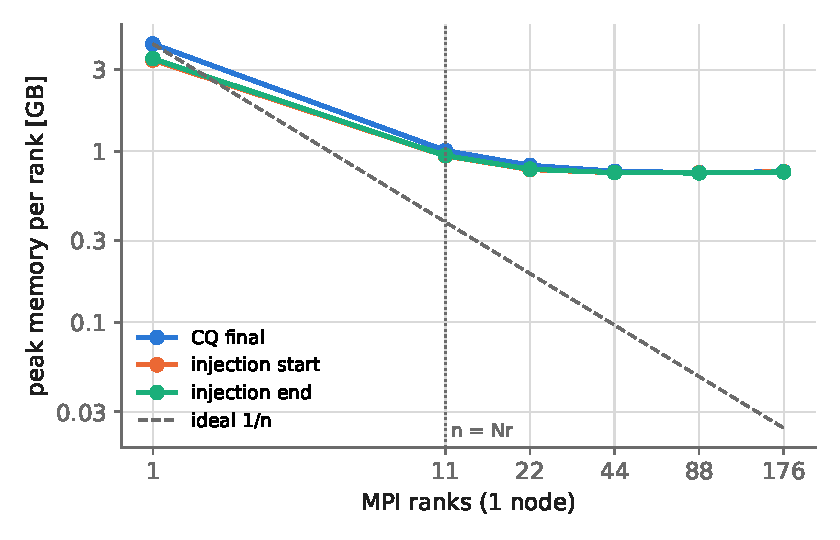
\includegraphics[width=\linewidth]{v3_2877888/fig_memory_scaling}
        \end{column}
        \begin{column}{0.42\textwidth}
            \small
            \begin{itemize}
                \item CQ final: 4.34\,GB (1 rank) $\to$ 1.03\,GB (11) $\to$ 0.78\,GB (176)
                \item \textbf{plateau at $\approx 0.78$\,GB} from 44 ranks on
                \item same behaviour for the 3 snapshots
                \item the distributed parts do scale:
                \begin{itemize}
                    \item solve (incl.\ AMG setup) 2.83\,GB $\to$ 33\,MB
                    \item PETSc matrix 463 $\to$ 5\,MB
                    \item coefficients 302 $\to$ 10\,MB
                \end{itemize}
                \item at 176 ranks: $\approx 134$\,GB per node, vs 4.3\,GB serial
            \end{itemize}
        \end{column}
    \end{columns}
\end{frame}

% ---------------------------------------------------------------------
\begin{frame}{Memory: whole run vs construction only}
    \begin{columns}[T]
        \begin{column}{0.58\textwidth}
            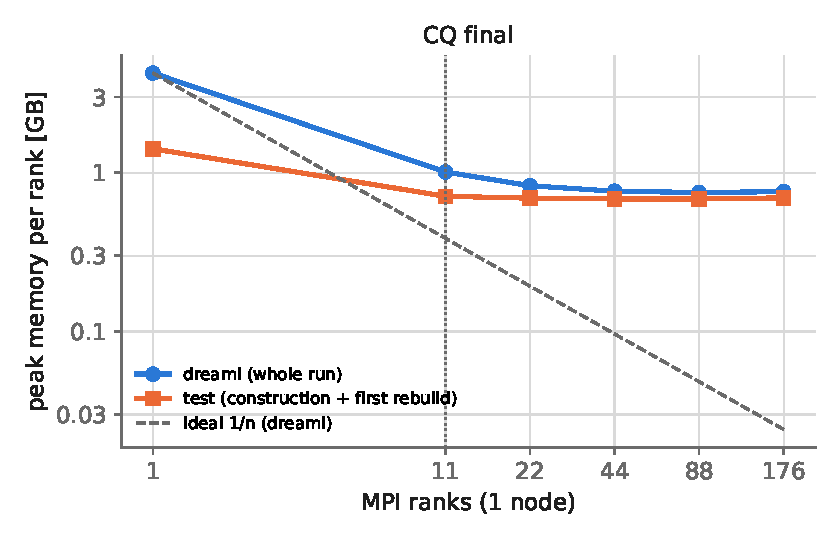
\includegraphics[width=\linewidth]{v3_2877888/memory_CQ_tf}
        \end{column}
        \begin{column}{0.42\textwidth}
            \small
            \begin{itemize}
                \item \textbf{test}: construction + first rebuild, no solve
                \begin{itemize}
                    \item 1.45\,GB $\to$ 0.71\,GB, flat from 11 ranks on
                \end{itemize}
                \item \textbf{dreami}: whole run
                \begin{itemize}
                    \item 4.34\,GB $\to$ 0.78\,GB
                \end{itemize}
                \item the gap between the two (the solve) shrinks with $n$:
                      the solver memory is distributed
                \item the plateau is already there after the construction:
                      the replicated data is created when the simulation is built
            \end{itemize}
        \end{column}
    \end{columns}
\end{frame}

% ---------------------------------------------------------------------
\begin{frame}{Where the memory of a rank goes}
    \begin{columns}[T]
        \begin{column}{0.56\textwidth}
            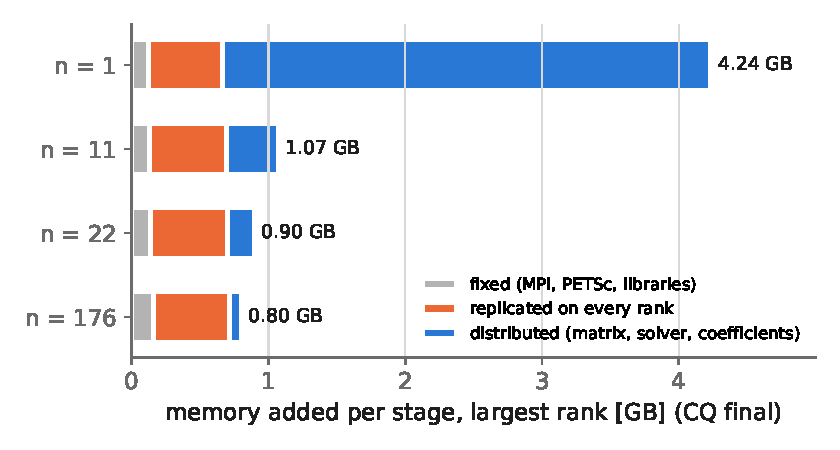
\includegraphics[width=\linewidth]{v3_2877888/fig_memory_breakdown}
        \end{column}
        \begin{column}{0.44\textwidth}
            \small
            Still \textbf{replicated} on every rank ($\approx 0.49$\,GB):
            \vspace{0.3em}

            \begin{tabular}{lrr}
                \hline
                & now & before \\
                \hline
                runaway grid data & 168\,MB & 374\,MB \\
                system setup (vectors) & 142\,MB & 142\,MB \\
                unknowns ($f$ history) & 71\,MB & 72\,MB \\
                equation terms & 64\,MB & 64\,MB \\
                hot-tail grid data & 46\,MB & 100\,MB \\
                output quantities & 0\,MB & 286\,MB \\
                \hline
            \end{tabular}
            \vspace{0.5em}

            Grid data: the metric $\sqrt{g}$ (one array per cell) is now
            computed when a bounce average needs it.
            Output: $\nu_s$, $\nu_D$ diagnostics removed
            (the solver's own $\nu_s$, $\nu_D$ are distributed)
            \vspace{0.3em}

            Above 22 ranks this is almost all of a rank's memory
        \end{column}
    \end{columns}
\end{frame}

% ---------------------------------------------------------------------
\begin{frame}{Speed-up}
    \begin{columns}[T]
        \begin{column}{0.5\textwidth}
            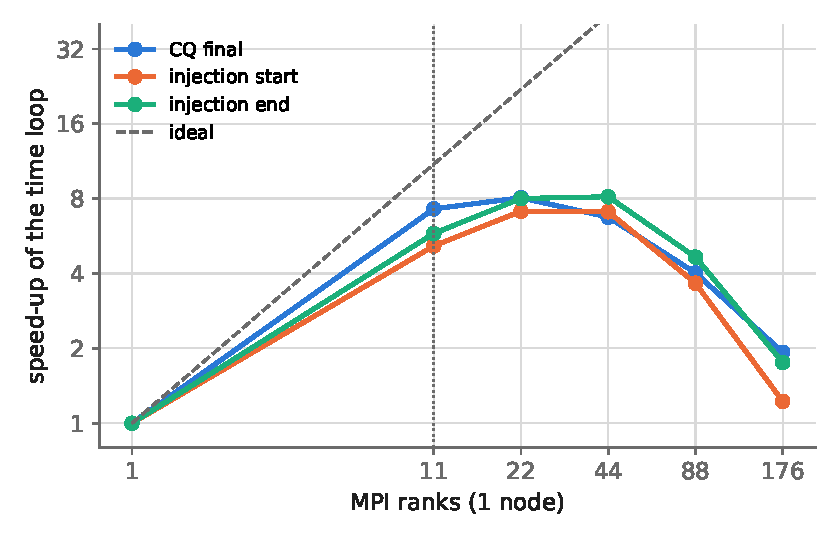
\includegraphics[width=\linewidth]{v3_2877888/fig_speedup}
            \centering{\footnotesize time loop, 3 snapshots}
        \end{column}
        \begin{column}{0.5\textwidth}
            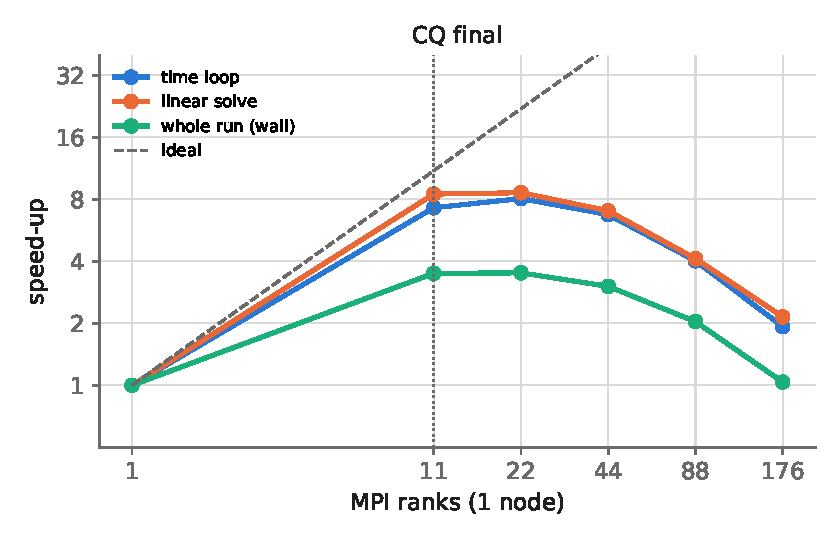
\includegraphics[width=\linewidth]{v3_2877888/speedup_CQ_tf}
            \centering{\footnotesize CQ final: loop, linear solve, whole run}
        \end{column}
    \end{columns}
    \vspace{0.3em}
    \small
    \begin{itemize}
        \item time loop: best at 22--44 ranks, $\approx 7$--$8\times$ (CQ final: 11.6\,s $\to$ 1.44\,s at 22 ranks)
        \item for $n > N_r$ each radius block is split over $n/N_r$ ranks:
              AMG/ILU setup dominated by communication
        \item whole run: at most $3.5\times$ (11--22 ranks), $1.0\times$ at 176 ranks
    \end{itemize}
\end{frame}

% ---------------------------------------------------------------------
\begin{frame}{Where the time goes (CQ final)}
    \begin{center}
        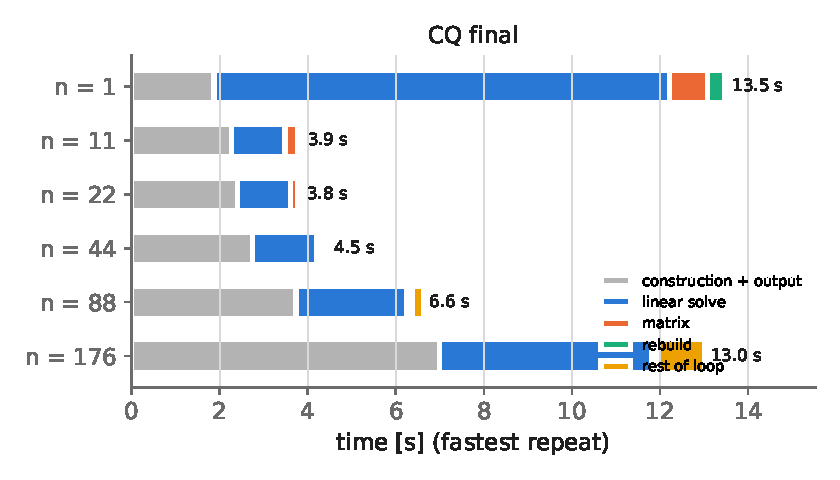
\includegraphics[width=0.85\linewidth]{v3_2877888/time_breakdown_CQ_tf}
    \end{center}
    \small
    \begin{itemize}
        \item 1 rank: 13.5\,s, of which 10.3\,s linear solve and 1.9\,s construction
        \item 22 ranks: 3.8\,s, the solve is down to 1.2\,s, the construction is 2.4\,s
        \item 176 ranks: 13.0\,s, construction 7.0\,s (replicated work, all ranks at the same time)
              and solve 4.8\,s (communication)
        \item \textbf{the construction does not scale}: same cause as the replicated memory
    \end{itemize}
\end{frame}

% ---------------------------------------------------------------------
\begin{frame}{Memory reduction step by step (CQ final, L2, $N_r = 11$)}
    \begin{center}
    \begin{tabular}{lccc}
        \hline
        & v1 & v2 & v3 \\
        & & no $\nu_s$, $\nu_D$ output & + metric on the fly \\
        \hline
        peak per rank, 1 rank      & 4.83\,GB & 4.59\,GB & 4.34\,GB \\
        peak per rank, 11 ranks    & 1.60\,GB & 1.30\,GB & 1.03\,GB \\
        peak per rank, 176 ranks   & 1.30\,GB & 1.04\,GB & \textbf{0.78\,GB} \\
        replicated per rank        & 1.1\,GB  & 0.75\,GB & \textbf{0.49\,GB} \\
        whole node, 176 ranks      & 225\,GB  & 180\,GB  & \textbf{134\,GB} \\
        time loop, 22 ranks        & 1.47\,s  & 1.43\,s  & 1.44\,s \\
        \hline
    \end{tabular}
    \end{center}
    \vspace{0.5em}
    \begin{itemize}
        \item $-40\,\%$ memory per rank at large $n$, same speed
        \item both removed parts grow with $N_r$: at $N_r = 44$ they were
              $\approx 2.2$\,GB per rank, the reason $N_r \geq 88$ did not fit on one node
    \end{itemize}
\end{frame}

% ---------------------------------------------------------------------
\begin{frame}{Conclusions and next steps}
    \begin{itemize}
        \item Distributed matrix, solver and coefficients: scale as expected
        \item \textbf{Still limited by replicated data}, now $\approx 0.49$\,GB per rank at L2
              (was 1.1\,GB): memory and construction time
        \item Best setting at L2: 11--22 ranks, $\approx 8\times$ speed-up of the time loop,
              0.85--1.03\,GB per rank
    \end{itemize}
    \vspace{0.5em}
    Next:
    \begin{enumerate}
        \item reduce replicated data: grid data left (214\,MB: phase-space volume,
              bounce averages, trapping flags), system vectors (142\,MB)
        \item more radial cells ($N_r > 11$): more independent blocks for the radial block Jacobi
        \item toroidal geometry (in progress): analytic shape fitted to the ITER equilibrium
              of the snapshots ($B_\mathrm{max}$ within 0.1\,\%), runs on 1 rank;
              the trapped-region boundary condition still has to be distributed
    \end{enumerate}
\end{frame}
 (update_2026-11-19.tex).

% ---------------------------------------------------------------------
\begin{frame}{Recent changes}
    \begin{itemize}
        \item \textbf{Memory distributed across MPI ranks}
        \begin{itemize}
            \item collision quantities ($\ln\Lambda$, $\nu_s$, $\nu_D$, $\nu_\parallel$) split by radius,
                  following the PETSc rows of $f_\mathrm{hot}$, $f_\mathrm{re}$
            \item partial derivatives no longer stored: computed cell by cell when needed
            \item kinetic operators (transient weights, advection/diffusion coefficients,
                  interpolation coefficients) stored only on the $\xi$-lines a rank owns
        \end{itemize}
        \item \textbf{Solver now handles the current-quench (CQ) snapshots}
        \begin{itemize}
            \item MIRadialBJ: each radius block uses BoomerAMG with a
                  Euclid ILU(1) smoother by default
            \item CQ at 29\,ms ($E \approx 31$\,V/m): failed with ILU(0),
                  now converges in 11 outer iterations
        \end{itemize}
        \item \textbf{Kinetic-only fluid unknowns} ($n_\mathrm{re}$, $j$, $n_\mathrm{tot}$)
              initialised by DREAM's own equations, then kept fixed
        \item \textbf{Memory and timing per stage} logged by \texttt{dreami}
              (\texttt{-dream\_log\_memory}) + batch script and summary
        \item \textbf{Replicated memory reduced}
        \begin{itemize}
            \item output diagnostics $\nu_s$, $\nu_D$ (full momentum grids) no longer saved: $-286$\,MB
            \item grid metric $\sqrt{g}$ computed when needed, not stored per cell
                  (cylindrical: no trapped orbits): $-260$\,MB
        \end{itemize}
    \end{itemize}
\end{frame}

% ---------------------------------------------------------------------
\begin{frame}{Correctness check}
    Reference: first kinetic-only version (serial) and unmodified DREAM, same settings
    \vspace{0.5em}
    \begin{center}
    \begin{tabular}{lcc}
        \hline
        comparison & $f_\mathrm{hot}$ & $f_\mathrm{re}$ \\
        \hline
        current code vs first kinetic-only version & $4\times10^{-9}$ & $1\times10^{-7}$ \\
        full DREAM (particle source off) vs first version & $6\times10^{-10}$ & $2\times10^{-14}$ \\
        \hline
    \end{tabular}
    \end{center}
    \vspace{0.5em}
    \begin{itemize}
        \item differences at the level of the iterative solver tolerance
        \item collision quantities: 1 rank vs $N$ ranks identical (difference exactly 0)
        \item only physics difference with full DREAM: the $f_\mathrm{hot}$ particle source,
              not included in kinetic-only mode ($\sim 8\times10^{-4}$ per step in $f_\mathrm{hot}$)
    \end{itemize}
\end{frame}

% ---------------------------------------------------------------------
\begin{frame}{Memory and speed-up test: setup}
    \begin{itemize}
        \item 3 snapshots of the ITER disruption: injection start, injection end, CQ final
        \item resolution level L2:
        \begin{itemize}
            \item hot-tail grid $500 \times 64$, runaway grid $300 \times 400$ ($p \times \xi$)
            \item $N_r = 11$ radii $\Rightarrow \approx 1.7$\,M unknowns
        \end{itemize}
        \item 1 time step, cylindrical geometry, linear solver MIRadialBJ
        \item Pitagora (CINECA), 1 node (256 cores), $n = 1, 11, 22, 44, 88, 176$ MPI ranks,
              2 runs each (fastest kept)
        \item measured per rank:
        \begin{itemize}
            \item resident memory at each stage (construction, matrix, solve)
            \item size of each distributed data structure
            \item time of the time loop, of the solve and of the whole run
        \end{itemize}
    \end{itemize}
\end{frame}

% ---------------------------------------------------------------------
\begin{frame}{Memory per rank}
    \begin{columns}[T]
        \begin{column}{0.58\textwidth}
            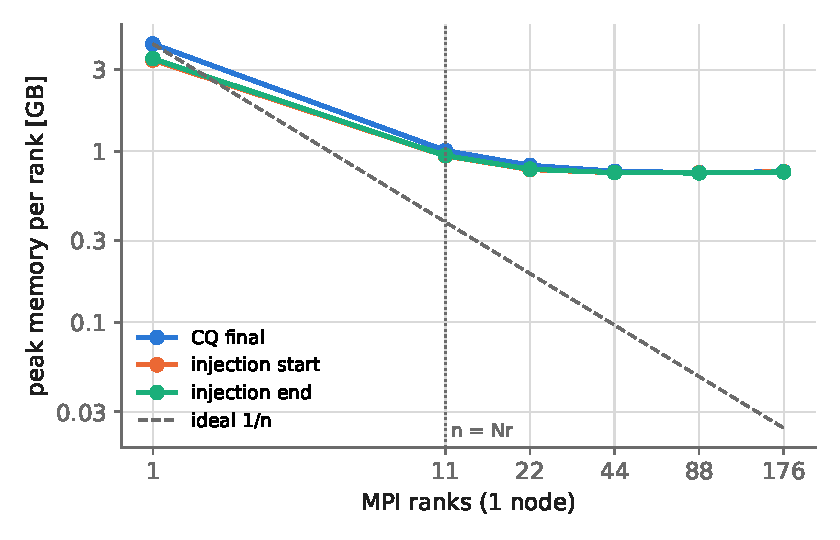
\includegraphics[width=\linewidth]{v3_2877888/fig_memory_scaling}
        \end{column}
        \begin{column}{0.42\textwidth}
            \small
            \begin{itemize}
                \item CQ final: 4.34\,GB (1 rank) $\to$ 1.03\,GB (11) $\to$ 0.78\,GB (176)
                \item \textbf{plateau at $\approx 0.78$\,GB} from 44 ranks on
                \item same behaviour for the 3 snapshots
                \item the distributed parts do scale:
                \begin{itemize}
                    \item solve (incl.\ AMG setup) 2.83\,GB $\to$ 33\,MB
                    \item PETSc matrix 463 $\to$ 5\,MB
                    \item coefficients 302 $\to$ 10\,MB
                \end{itemize}
                \item at 176 ranks: $\approx 134$\,GB per node, vs 4.3\,GB serial
            \end{itemize}
        \end{column}
    \end{columns}
\end{frame}

% ---------------------------------------------------------------------
\begin{frame}{Memory: whole run vs construction only}
    \begin{columns}[T]
        \begin{column}{0.58\textwidth}
            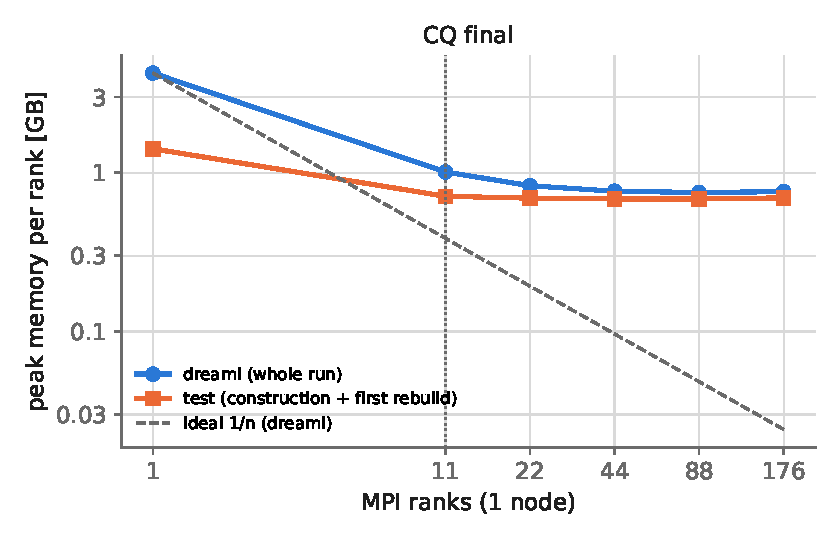
\includegraphics[width=\linewidth]{v3_2877888/memory_CQ_tf}
        \end{column}
        \begin{column}{0.42\textwidth}
            \small
            \begin{itemize}
                \item \textbf{test}: construction + first rebuild, no solve
                \begin{itemize}
                    \item 1.45\,GB $\to$ 0.71\,GB, flat from 11 ranks on
                \end{itemize}
                \item \textbf{dreami}: whole run
                \begin{itemize}
                    \item 4.34\,GB $\to$ 0.78\,GB
                \end{itemize}
                \item the gap between the two (the solve) shrinks with $n$:
                      the solver memory is distributed
                \item the plateau is already there after the construction:
                      the replicated data is created when the simulation is built
            \end{itemize}
        \end{column}
    \end{columns}
\end{frame}

% ---------------------------------------------------------------------
\begin{frame}{Where the memory of a rank goes}
    \begin{columns}[T]
        \begin{column}{0.56\textwidth}
            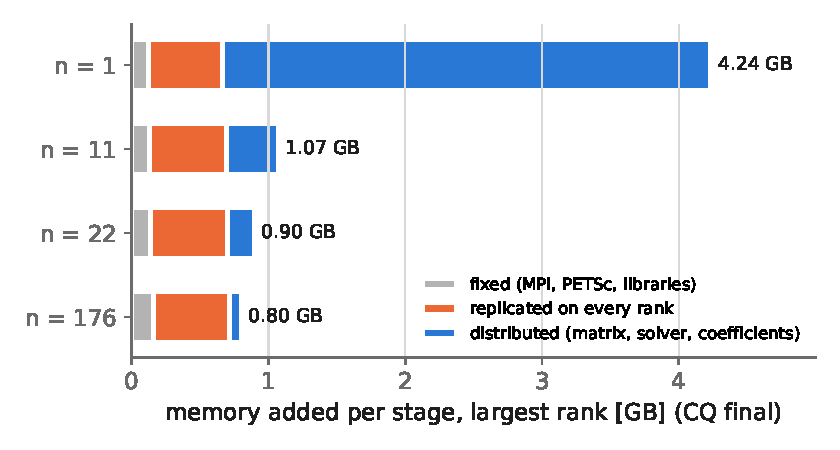
\includegraphics[width=\linewidth]{v3_2877888/fig_memory_breakdown}
        \end{column}
        \begin{column}{0.44\textwidth}
            \small
            Still \textbf{replicated} on every rank ($\approx 0.49$\,GB):
            \vspace{0.3em}

            \begin{tabular}{lrr}
                \hline
                & now & before \\
                \hline
                runaway grid data & 168\,MB & 374\,MB \\
                system setup (vectors) & 142\,MB & 142\,MB \\
                unknowns ($f$ history) & 71\,MB & 72\,MB \\
                equation terms & 64\,MB & 64\,MB \\
                hot-tail grid data & 46\,MB & 100\,MB \\
                output quantities & 0\,MB & 286\,MB \\
                \hline
            \end{tabular}
            \vspace{0.5em}

            Grid data: the metric $\sqrt{g}$ (one array per cell) is now
            computed when a bounce average needs it.
            Output: $\nu_s$, $\nu_D$ diagnostics removed
            (the solver's own $\nu_s$, $\nu_D$ are distributed)
            \vspace{0.3em}

            Above 22 ranks this is almost all of a rank's memory
        \end{column}
    \end{columns}
\end{frame}

% ---------------------------------------------------------------------
\begin{frame}{Speed-up}
    \begin{columns}[T]
        \begin{column}{0.5\textwidth}
            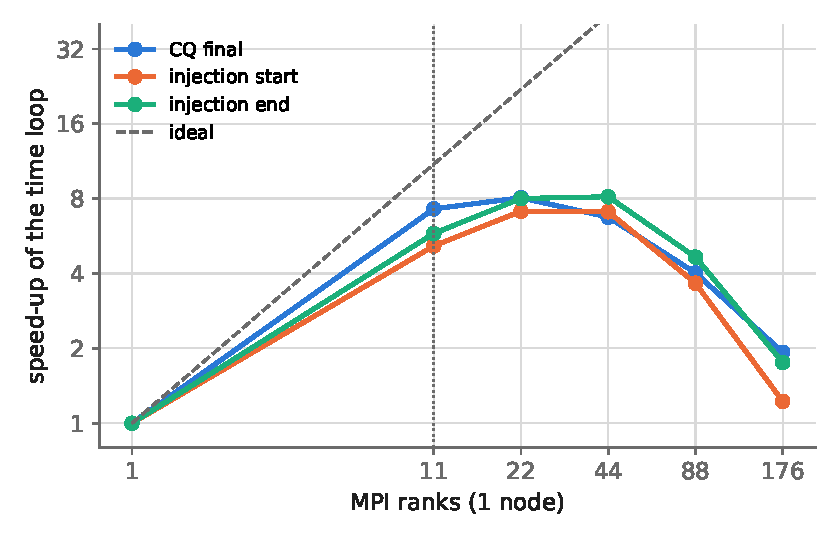
\includegraphics[width=\linewidth]{v3_2877888/fig_speedup}
            \centering{\footnotesize time loop, 3 snapshots}
        \end{column}
        \begin{column}{0.5\textwidth}
            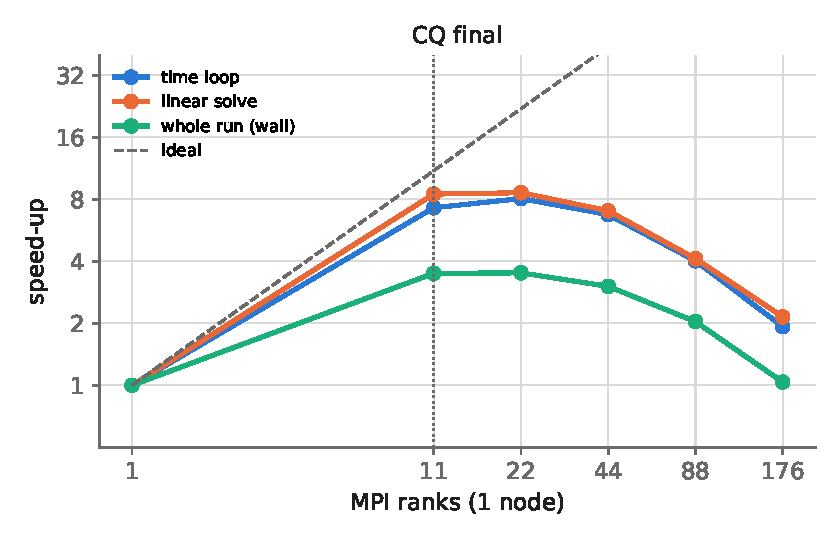
\includegraphics[width=\linewidth]{v3_2877888/speedup_CQ_tf}
            \centering{\footnotesize CQ final: loop, linear solve, whole run}
        \end{column}
    \end{columns}
    \vspace{0.3em}
    \small
    \begin{itemize}
        \item time loop: best at 22--44 ranks, $\approx 7$--$8\times$ (CQ final: 11.6\,s $\to$ 1.44\,s at 22 ranks)
        \item for $n > N_r$ each radius block is split over $n/N_r$ ranks:
              AMG/ILU setup dominated by communication
        \item whole run: at most $3.5\times$ (11--22 ranks), $1.0\times$ at 176 ranks
    \end{itemize}
\end{frame}

% ---------------------------------------------------------------------
\begin{frame}{Where the time goes (CQ final)}
    \begin{center}
        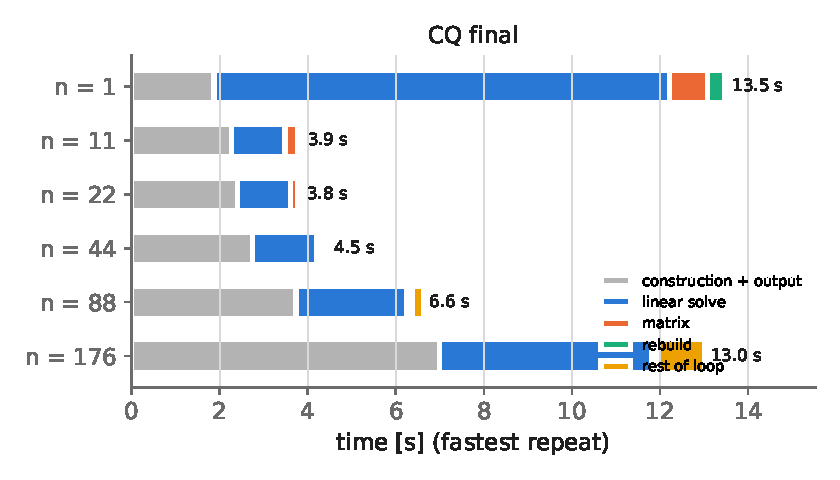
\includegraphics[width=0.85\linewidth]{v3_2877888/time_breakdown_CQ_tf}
    \end{center}
    \small
    \begin{itemize}
        \item 1 rank: 13.5\,s, of which 10.3\,s linear solve and 1.9\,s construction
        \item 22 ranks: 3.8\,s, the solve is down to 1.2\,s, the construction is 2.4\,s
        \item 176 ranks: 13.0\,s, construction 7.0\,s (replicated work, all ranks at the same time)
              and solve 4.8\,s (communication)
        \item \textbf{the construction does not scale}: same cause as the replicated memory
    \end{itemize}
\end{frame}

% ---------------------------------------------------------------------
\begin{frame}{Memory reduction step by step (CQ final, L2, $N_r = 11$)}
    \begin{center}
    \begin{tabular}{lccc}
        \hline
        & v1 & v2 & v3 \\
        & & no $\nu_s$, $\nu_D$ output & + metric on the fly \\
        \hline
        peak per rank, 1 rank      & 4.83\,GB & 4.59\,GB & 4.34\,GB \\
        peak per rank, 11 ranks    & 1.60\,GB & 1.30\,GB & 1.03\,GB \\
        peak per rank, 176 ranks   & 1.30\,GB & 1.04\,GB & \textbf{0.78\,GB} \\
        replicated per rank        & 1.1\,GB  & 0.75\,GB & \textbf{0.49\,GB} \\
        whole node, 176 ranks      & 225\,GB  & 180\,GB  & \textbf{134\,GB} \\
        time loop, 22 ranks        & 1.47\,s  & 1.43\,s  & 1.44\,s \\
        \hline
    \end{tabular}
    \end{center}
    \vspace{0.5em}
    \begin{itemize}
        \item $-40\,\%$ memory per rank at large $n$, same speed
        \item both removed parts grow with $N_r$: at $N_r = 44$ they were
              $\approx 2.2$\,GB per rank, the reason $N_r \geq 88$ did not fit on one node
    \end{itemize}
\end{frame}

% ---------------------------------------------------------------------
\begin{frame}{Conclusions and next steps}
    \begin{itemize}
        \item Distributed matrix, solver and coefficients: scale as expected
        \item \textbf{Still limited by replicated data}, now $\approx 0.49$\,GB per rank at L2
              (was 1.1\,GB): memory and construction time
        \item Best setting at L2: 11--22 ranks, $\approx 8\times$ speed-up of the time loop,
              0.85--1.03\,GB per rank
    \end{itemize}
    \vspace{0.5em}
    Next:
    \begin{enumerate}
        \item reduce replicated data: grid data left (214\,MB: phase-space volume,
              bounce averages, trapping flags), system vectors (142\,MB)
        \item more radial cells ($N_r > 11$): more independent blocks for the radial block Jacobi
        \item toroidal geometry (in progress): analytic shape fitted to the ITER equilibrium
              of the snapshots ($B_\mathrm{max}$ within 0.1\,\%), runs on 1 rank;
              the trapped-region boundary condition still has to be distributed
    \end{enumerate}
\end{frame}
 (update_2026-11-19.tex).

% ---------------------------------------------------------------------
\begin{frame}{Recent changes}
    \begin{itemize}
        \item \textbf{Memory distributed across MPI ranks}
        \begin{itemize}
            \item collision quantities ($\ln\Lambda$, $\nu_s$, $\nu_D$, $\nu_\parallel$) split by radius,
                  following the PETSc rows of $f_\mathrm{hot}$, $f_\mathrm{re}$
            \item partial derivatives no longer stored: computed cell by cell when needed
            \item kinetic operators (transient weights, advection/diffusion coefficients,
                  interpolation coefficients) stored only on the $\xi$-lines a rank owns
        \end{itemize}
        \item \textbf{Solver now handles the current-quench (CQ) snapshots}
        \begin{itemize}
            \item MIRadialBJ: each radius block uses BoomerAMG with a
                  Euclid ILU(1) smoother by default
            \item CQ at 29\,ms ($E \approx 31$\,V/m): failed with ILU(0),
                  now converges in 11 outer iterations
        \end{itemize}
        \item \textbf{Kinetic-only fluid unknowns} ($n_\mathrm{re}$, $j$, $n_\mathrm{tot}$)
              initialised by DREAM's own equations, then kept fixed
        \item \textbf{Memory and timing per stage} logged by \texttt{dreami}
              (\texttt{-dream\_log\_memory}) + batch script and summary
        \item \textbf{Replicated memory reduced}
        \begin{itemize}
            \item output diagnostics $\nu_s$, $\nu_D$ (full momentum grids) no longer saved: $-286$\,MB
            \item grid metric $\sqrt{g}$ computed when needed, not stored per cell
                  (cylindrical: no trapped orbits): $-260$\,MB
        \end{itemize}
    \end{itemize}
\end{frame}

% ---------------------------------------------------------------------
\begin{frame}{Correctness check}
    Reference: first kinetic-only version (serial) and unmodified DREAM, same settings
    \vspace{0.5em}
    \begin{center}
    \begin{tabular}{lcc}
        \hline
        comparison & $f_\mathrm{hot}$ & $f_\mathrm{re}$ \\
        \hline
        current code vs first kinetic-only version & $4\times10^{-9}$ & $1\times10^{-7}$ \\
        full DREAM (particle source off) vs first version & $6\times10^{-10}$ & $2\times10^{-14}$ \\
        \hline
    \end{tabular}
    \end{center}
    \vspace{0.5em}
    \begin{itemize}
        \item differences at the level of the iterative solver tolerance
        \item collision quantities: 1 rank vs $N$ ranks identical (difference exactly 0)
        \item only physics difference with full DREAM: the $f_\mathrm{hot}$ particle source,
              not included in kinetic-only mode ($\sim 8\times10^{-4}$ per step in $f_\mathrm{hot}$)
    \end{itemize}
\end{frame}

% ---------------------------------------------------------------------
\begin{frame}{Memory and speed-up test: setup}
    \begin{itemize}
        \item 3 snapshots of the ITER disruption: injection start, injection end, CQ final
        \item resolution level L2:
        \begin{itemize}
            \item hot-tail grid $500 \times 64$, runaway grid $300 \times 400$ ($p \times \xi$)
            \item $N_r = 11$ radii $\Rightarrow \approx 1.7$\,M unknowns
        \end{itemize}
        \item 1 time step, cylindrical geometry, linear solver MIRadialBJ
        \item Pitagora (CINECA), 1 node (256 cores), $n = 1, 11, 22, 44, 88, 176$ MPI ranks,
              2 runs each (fastest kept)
        \item measured per rank:
        \begin{itemize}
            \item resident memory at each stage (construction, matrix, solve)
            \item size of each distributed data structure
            \item time of the time loop, of the solve and of the whole run
        \end{itemize}
    \end{itemize}
\end{frame}

% ---------------------------------------------------------------------
\begin{frame}{Memory per rank}
    \begin{columns}[T]
        \begin{column}{0.58\textwidth}
            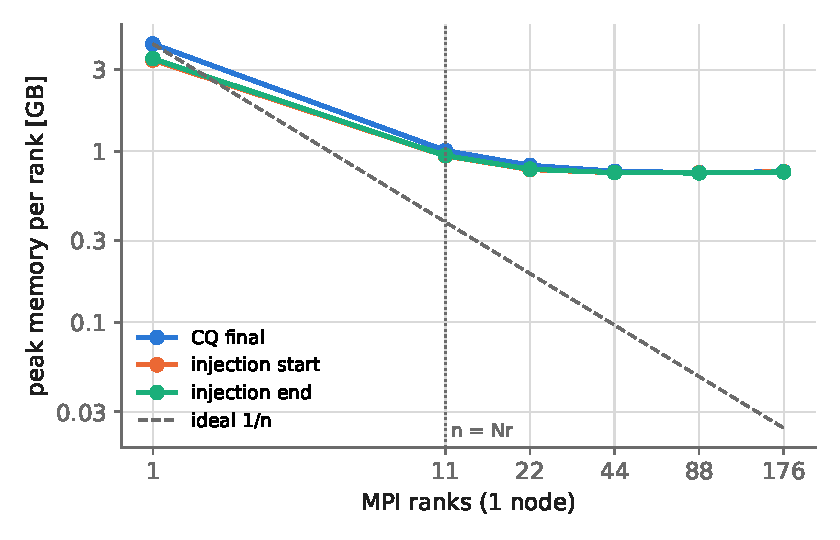
\includegraphics[width=\linewidth]{v3_2877888/fig_memory_scaling}
        \end{column}
        \begin{column}{0.42\textwidth}
            \small
            \begin{itemize}
                \item CQ final: 4.34\,GB (1 rank) $\to$ 1.03\,GB (11) $\to$ 0.78\,GB (176)
                \item \textbf{plateau at $\approx 0.78$\,GB} from 44 ranks on
                \item same behaviour for the 3 snapshots
                \item the distributed parts do scale:
                \begin{itemize}
                    \item solve (incl.\ AMG setup) 2.83\,GB $\to$ 33\,MB
                    \item PETSc matrix 463 $\to$ 5\,MB
                    \item coefficients 302 $\to$ 10\,MB
                \end{itemize}
                \item at 176 ranks: $\approx 134$\,GB per node, vs 4.3\,GB serial
            \end{itemize}
        \end{column}
    \end{columns}
\end{frame}

% ---------------------------------------------------------------------
\begin{frame}{Memory: whole run vs construction only}
    \begin{columns}[T]
        \begin{column}{0.58\textwidth}
            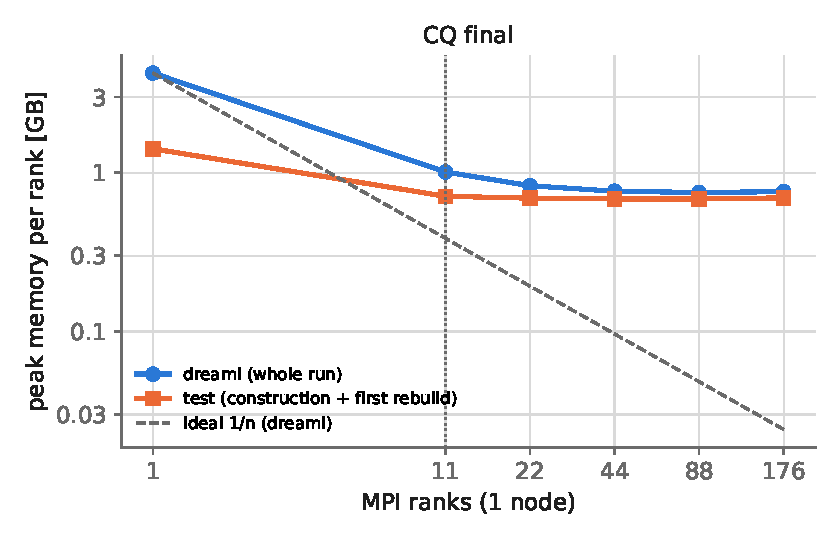
\includegraphics[width=\linewidth]{v3_2877888/memory_CQ_tf}
        \end{column}
        \begin{column}{0.42\textwidth}
            \small
            \begin{itemize}
                \item \textbf{test}: construction + first rebuild, no solve
                \begin{itemize}
                    \item 1.45\,GB $\to$ 0.71\,GB, flat from 11 ranks on
                \end{itemize}
                \item \textbf{dreami}: whole run
                \begin{itemize}
                    \item 4.34\,GB $\to$ 0.78\,GB
                \end{itemize}
                \item the gap between the two (the solve) shrinks with $n$:
                      the solver memory is distributed
                \item the plateau is already there after the construction:
                      the replicated data is created when the simulation is built
            \end{itemize}
        \end{column}
    \end{columns}
\end{frame}

% ---------------------------------------------------------------------
\begin{frame}{Where the memory of a rank goes}
    \begin{columns}[T]
        \begin{column}{0.56\textwidth}
            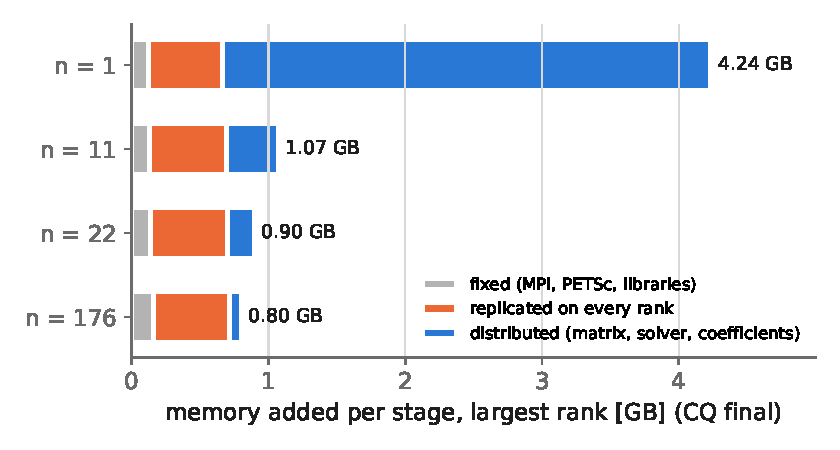
\includegraphics[width=\linewidth]{v3_2877888/fig_memory_breakdown}
        \end{column}
        \begin{column}{0.44\textwidth}
            \small
            Still \textbf{replicated} on every rank ($\approx 0.49$\,GB):
            \vspace{0.3em}

            \begin{tabular}{lrr}
                \hline
                & now & before \\
                \hline
                runaway grid data & 168\,MB & 374\,MB \\
                system setup (vectors) & 142\,MB & 142\,MB \\
                unknowns ($f$ history) & 71\,MB & 72\,MB \\
                equation terms & 64\,MB & 64\,MB \\
                hot-tail grid data & 46\,MB & 100\,MB \\
                output quantities & 0\,MB & 286\,MB \\
                \hline
            \end{tabular}
            \vspace{0.5em}

            Grid data: the metric $\sqrt{g}$ (one array per cell) is now
            computed when a bounce average needs it.
            Output: $\nu_s$, $\nu_D$ diagnostics removed
            (the solver's own $\nu_s$, $\nu_D$ are distributed)
            \vspace{0.3em}

            Above 22 ranks this is almost all of a rank's memory
        \end{column}
    \end{columns}
\end{frame}

% ---------------------------------------------------------------------
\begin{frame}{Speed-up}
    \begin{columns}[T]
        \begin{column}{0.5\textwidth}
            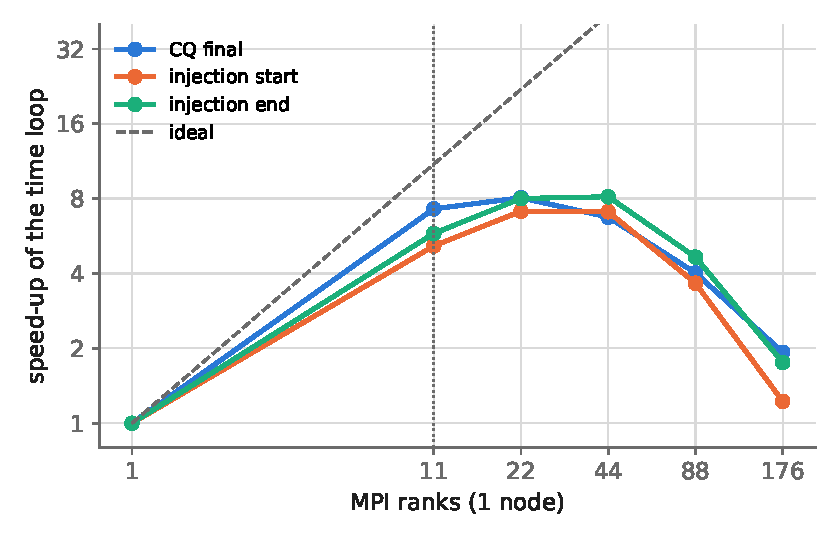
\includegraphics[width=\linewidth]{v3_2877888/fig_speedup}
            \centering{\footnotesize time loop, 3 snapshots}
        \end{column}
        \begin{column}{0.5\textwidth}
            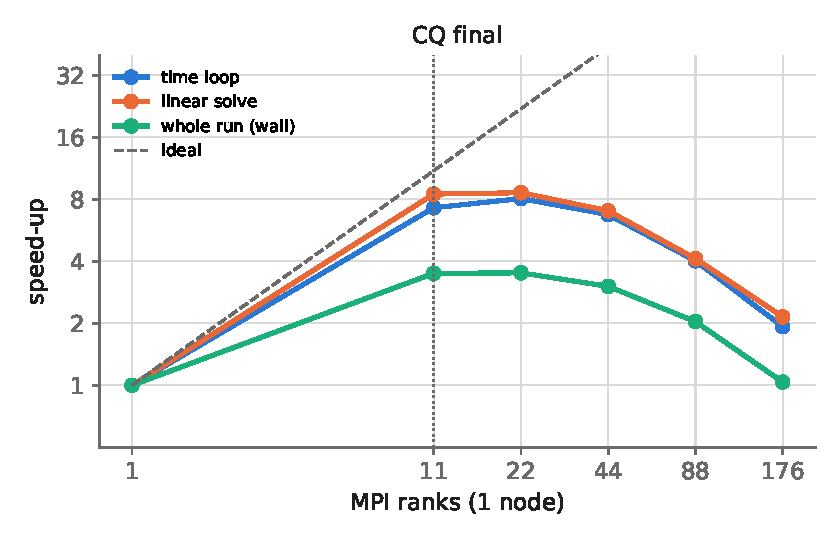
\includegraphics[width=\linewidth]{v3_2877888/speedup_CQ_tf}
            \centering{\footnotesize CQ final: loop, linear solve, whole run}
        \end{column}
    \end{columns}
    \vspace{0.3em}
    \small
    \begin{itemize}
        \item time loop: best at 22--44 ranks, $\approx 7$--$8\times$ (CQ final: 11.6\,s $\to$ 1.44\,s at 22 ranks)
        \item for $n > N_r$ each radius block is split over $n/N_r$ ranks:
              AMG/ILU setup dominated by communication
        \item whole run: at most $3.5\times$ (11--22 ranks), $1.0\times$ at 176 ranks
    \end{itemize}
\end{frame}

% ---------------------------------------------------------------------
\begin{frame}{Where the time goes (CQ final)}
    \begin{center}
        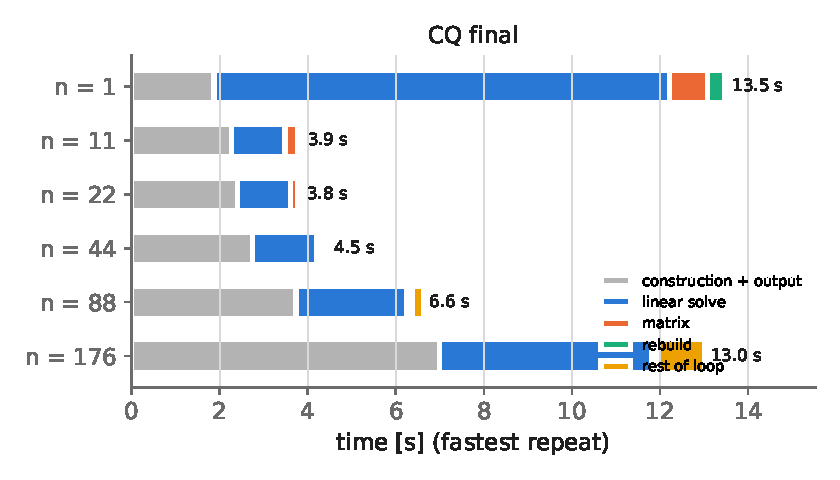
\includegraphics[width=0.85\linewidth]{v3_2877888/time_breakdown_CQ_tf}
    \end{center}
    \small
    \begin{itemize}
        \item 1 rank: 13.5\,s, of which 10.3\,s linear solve and 1.9\,s construction
        \item 22 ranks: 3.8\,s, the solve is down to 1.2\,s, the construction is 2.4\,s
        \item 176 ranks: 13.0\,s, construction 7.0\,s (replicated work, all ranks at the same time)
              and solve 4.8\,s (communication)
        \item \textbf{the construction does not scale}: same cause as the replicated memory
    \end{itemize}
\end{frame}

% ---------------------------------------------------------------------
\begin{frame}{Memory reduction step by step (CQ final, L2, $N_r = 11$)}
    \begin{center}
    \begin{tabular}{lccc}
        \hline
        & v1 & v2 & v3 \\
        & & no $\nu_s$, $\nu_D$ output & + metric on the fly \\
        \hline
        peak per rank, 1 rank      & 4.83\,GB & 4.59\,GB & 4.34\,GB \\
        peak per rank, 11 ranks    & 1.60\,GB & 1.30\,GB & 1.03\,GB \\
        peak per rank, 176 ranks   & 1.30\,GB & 1.04\,GB & \textbf{0.78\,GB} \\
        replicated per rank        & 1.1\,GB  & 0.75\,GB & \textbf{0.49\,GB} \\
        whole node, 176 ranks      & 225\,GB  & 180\,GB  & \textbf{134\,GB} \\
        time loop, 22 ranks        & 1.47\,s  & 1.43\,s  & 1.44\,s \\
        \hline
    \end{tabular}
    \end{center}
    \vspace{0.5em}
    \begin{itemize}
        \item $-40\,\%$ memory per rank at large $n$, same speed
        \item both removed parts grow with $N_r$: at $N_r = 44$ they were
              $\approx 2.2$\,GB per rank, the reason $N_r \geq 88$ did not fit on one node
    \end{itemize}
\end{frame}

% ---------------------------------------------------------------------
\begin{frame}{Conclusions and next steps}
    \begin{itemize}
        \item Distributed matrix, solver and coefficients: scale as expected
        \item \textbf{Still limited by replicated data}, now $\approx 0.49$\,GB per rank at L2
              (was 1.1\,GB): memory and construction time
        \item Best setting at L2: 11--22 ranks, $\approx 8\times$ speed-up of the time loop,
              0.85--1.03\,GB per rank
    \end{itemize}
    \vspace{0.5em}
    Next:
    \begin{enumerate}
        \item reduce replicated data: grid data left (214\,MB: phase-space volume,
              bounce averages, trapping flags), system vectors (142\,MB)
        \item more radial cells ($N_r > 11$): more independent blocks for the radial block Jacobi
        \item toroidal geometry (in progress): analytic shape fitted to the ITER equilibrium
              of the snapshots ($B_\mathrm{max}$ within 0.1\,\%), runs on 1 rank;
              the trapped-region boundary condition still has to be distributed
    \end{enumerate}
\end{frame}
